\chapter{Modbus RTU}
\label{Anhang:Modbus}

Abbild \ref{fig:Bit} zeigt die zwei Bit-Sequenzen exemplarisch auf. 

\begin{figure}[htb]
\centering
\subfigure[Bit-Sequenz in RTU-Mode]
{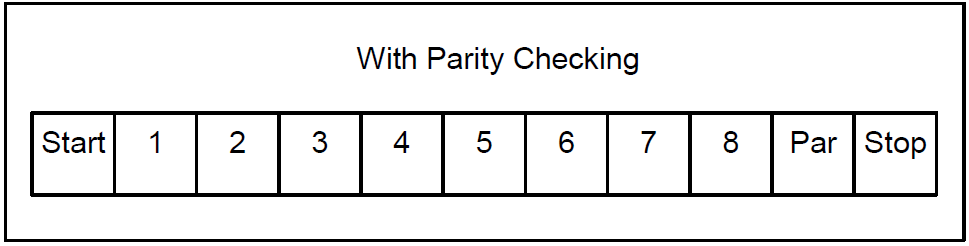
\includegraphics[width=0.7\textwidth]
{Pictures/Versuchsaufbau/bitsequenz1.png}}
%\hspace{1cm}
\subfigure[Bit-Sequenz in RTU-Modbus ohne Paritätsbit mit zusätzlichem Stopbit]{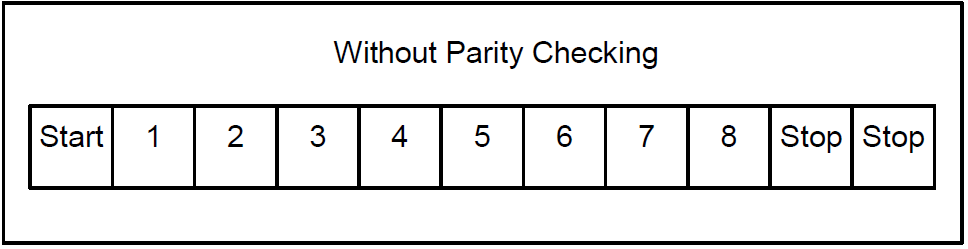
\includegraphics[width=0.7\textwidth]
{Pictures/Versuchsaufbau/bitsequenz2.png}}
\caption{Verschiedene Bit-Sequenzen im RTU-Modus \citep{MODBUS.ORG2002}}
\label{fig:Bit}
\end{figure}

\begin{table}[htb]
\centering
\caption{Modbus-Register Adressen \citep{KMGH2013}}
\begin{tabular}{lll}
\hline 
\textbf{Adressbereich} & \textbf{Zwischenspeicher} & \textbf{Zugriffsrechten} \\ 
\hline 
\hline 
0\dots 9999 & Coils & lesen + schreiben \\ 
\hline 
10000\dots 19999 & Discrete Inputs & lesen \\ 
\hline 
20000\dots 39999 & Input Registers & lesen \\ 
\hline 
40000\dots 65535 & Holding Registers & lesen + schreiben \\ 
\hline 
\hline 
\end{tabular} 
\label{tab:modbus_registers}
\end{table}


\begin{table}[htb]
\centering
\caption{Modbus-Befehle mit ihrem Funktions-Code }
\begin{tabular}{ll}
\hline 
\textbf{Funktions-Code (in Dezimalsystem)} & \textbf{Befehl} \\ 
\hline 
\hline
01 & Read Single Coil \\ 
\hline 
02 & Read Descrete Inputs \\ 
\hline 
03 & Read Holding Register \\ 
\hline 
04 & Read Input Register \\ 
\hline 
05 & Write Single Coil \\ 
\hline 
08 & Diagnostics \\ 
\hline 
16 & Write Multiple Register \\ 
\hline 
\hline 
\end{tabular} 
\label{tab:modbus_befehle}
\end{table}

\begin{table}[htb]
\centering
\caption{Datenleitungsbezeichnungen für RS485 }
\begin{tabular}{p{3cm}p{3cm}llllll}
\hline 
\rule[-1ex]{0pt}{2.5ex} \textbf{Modbus Org.} & \textbf{EIA/TIA-485 Standard} & \textbf{Beckhoff/ TwinCat} & \textbf{\textsc{Keller}} & \textbf{\textsc{Krohne}} & \textbf{\textsc{Carel}} \\ 
\hline 
\hline 
\rule[-1ex]{0pt}{2.5ex} D0 & Data A = Data (-) = inverted & Data (-) & RS 485 B & Signal A (D0) & (-) \\ 
\hline 
\rule[-1ex]{0pt}{2.5ex} D1 & Data B = Data (+) = non-inverted & Data (+) & RS 485 A & Signal B (D1) & (+) \\ 
\hline 
\rule[-1ex]{0pt}{2.5ex} Common & Common & Ground & GND & Common & GND \\ 
\hline 
\hline 
\end{tabular} 
\end{table}



\chapter{Risikomanagementanalyse}



\begin{figure}[htb]
\centering
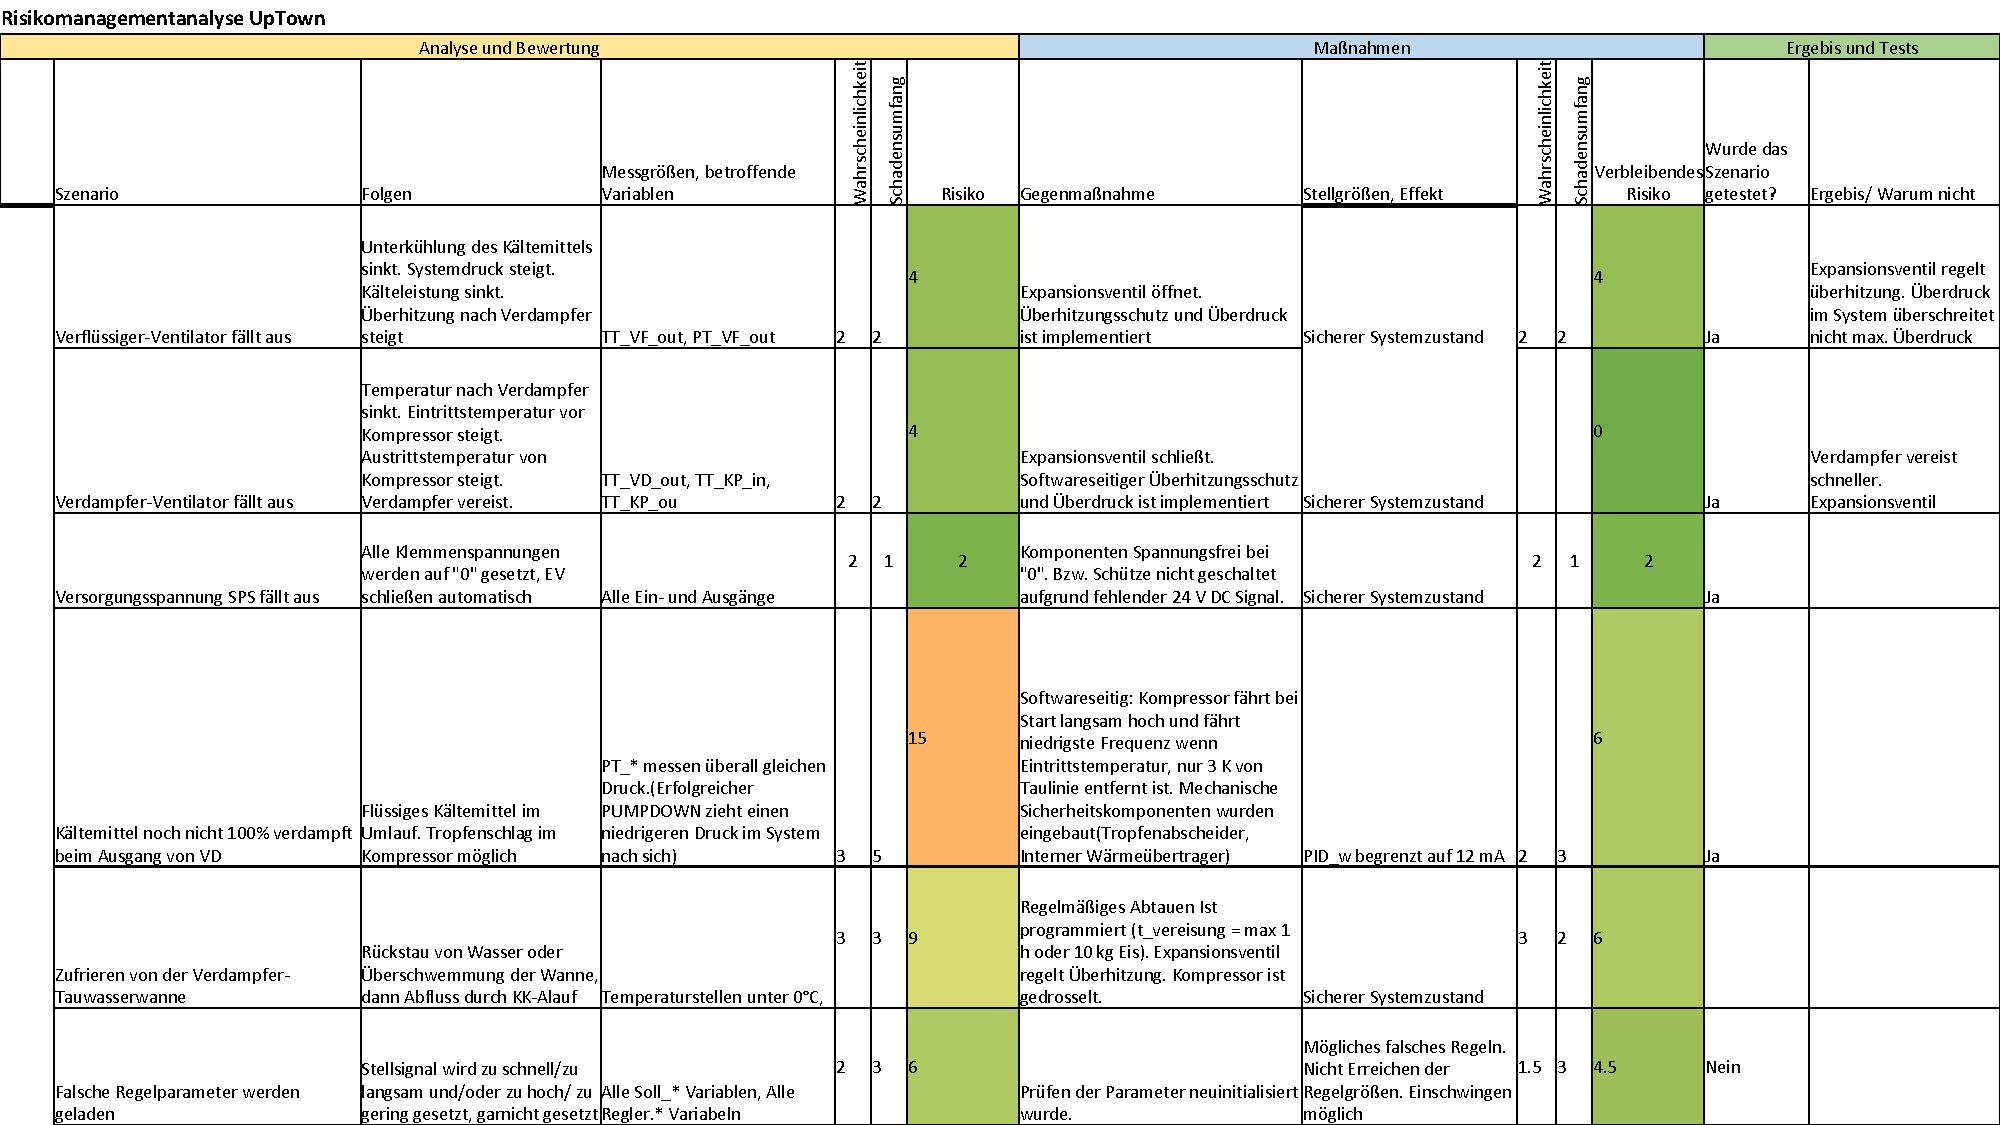
\includegraphics[page= 1, width=1.35\textwidth, angle = 90]
{Pictures/Anhang/Riskikomanagementanalyse.pdf}
\caption{(a): Risikomanagementanalyse nach ISO 31000}
\label{fig:}
\end{figure}



\begin{figure}[htb]
\centering
\includegraphics[page=2, width=1.35\textwidth, angle = 90]
{Pictures/Anhang/Riskikomanagementanalyse.pdf}
\caption{(b): Risikomanagementanalyse nach ISO 31000}
\label{fig:}
\end{figure}


\chapter{Programmabläufe bei Abtaumethoden}

\begin{figure}[htb]
\centering
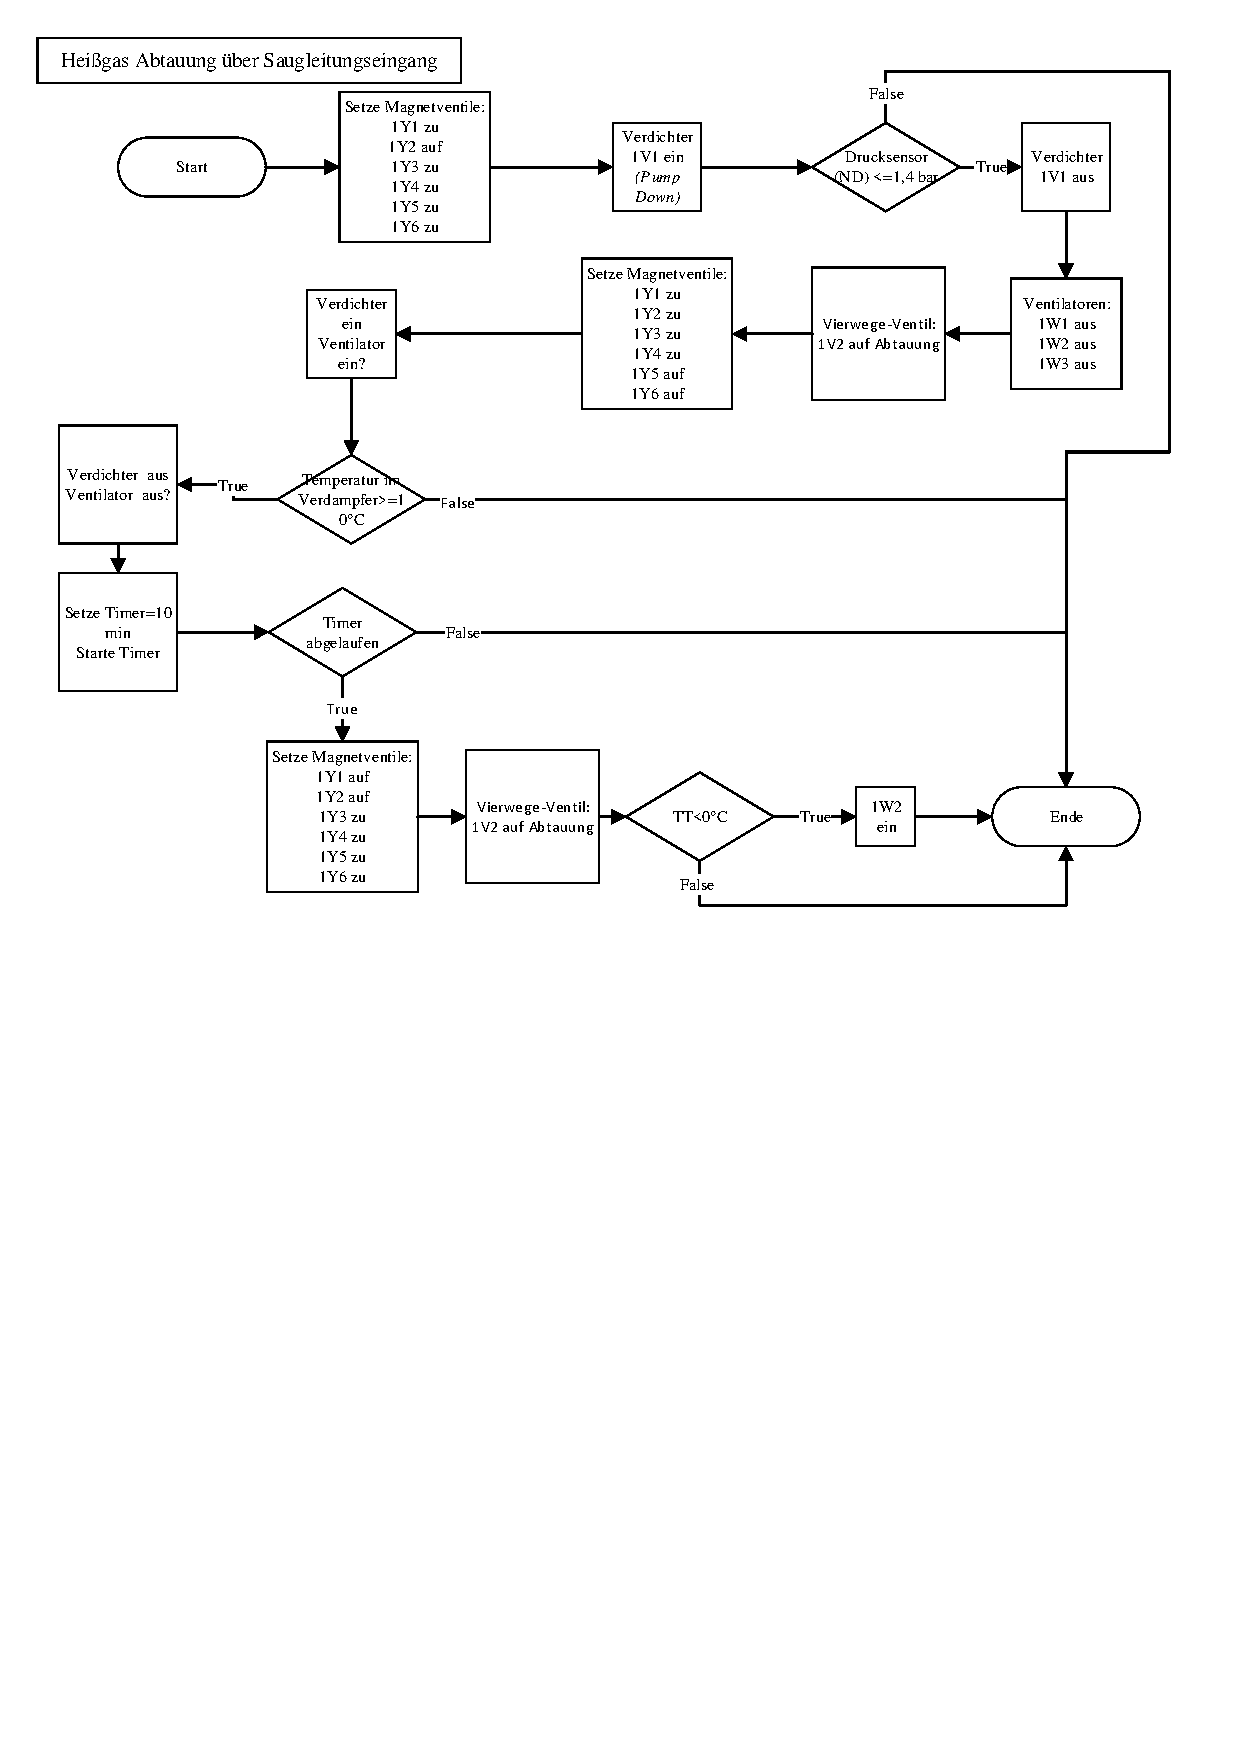
\includegraphics[width=0.9\textwidth]
{Pictures/Anhang/Ablauf_HG_Saugleitung.pdf}
\caption{Heißgas-Abtauung über Saugleitung}
\label{fig:}
\end{figure}


\begin{figure}[htb]
\centering
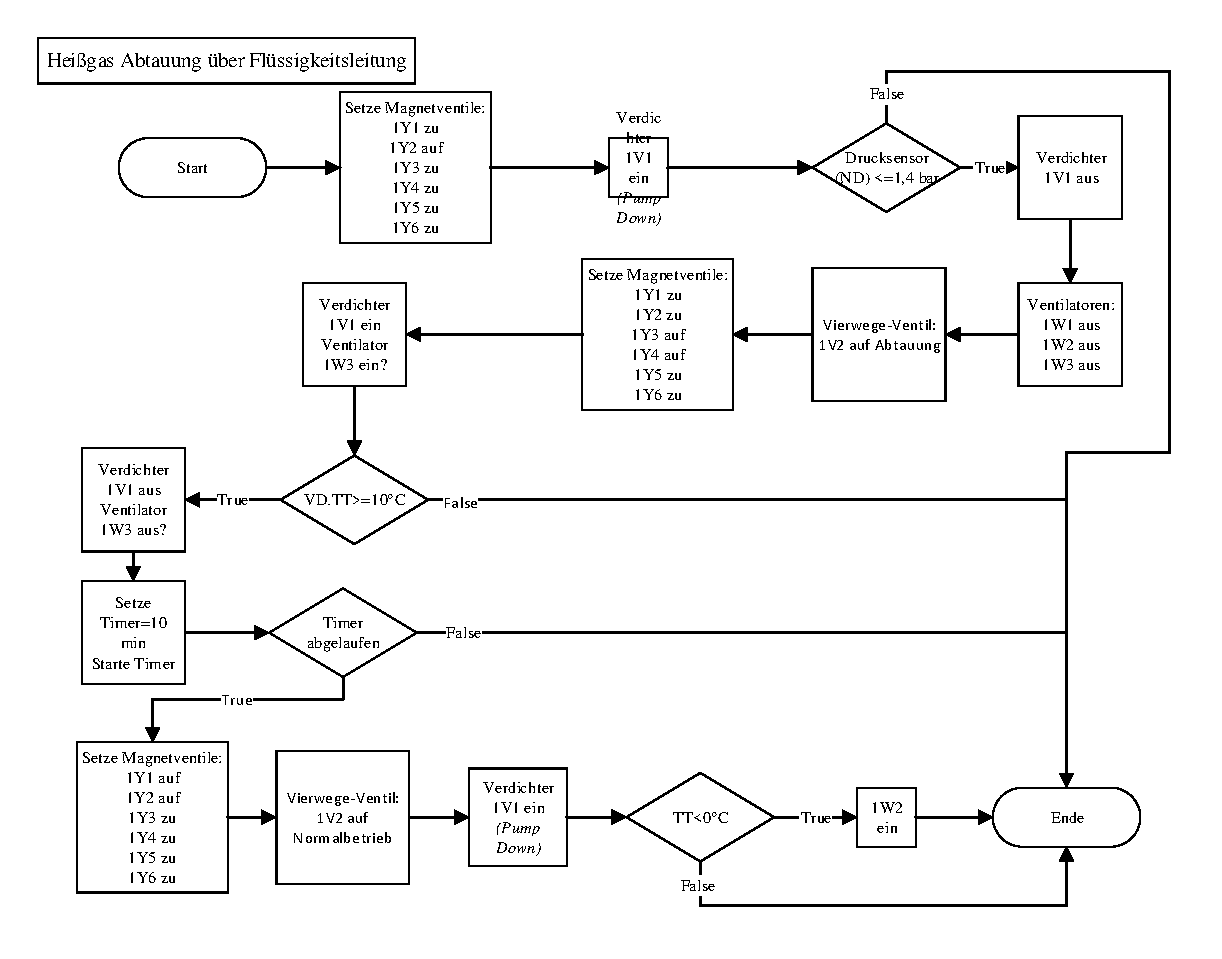
\includegraphics[ width=1.\textwidth]
{Pictures/Anhang/Abtauen_HG_Flussig.pdf}
\caption{Heißgas-Abtauung über Flüssigkeitleitung}
\label{fig:}
\end{figure}


\begin{figure}[htb]
\centering
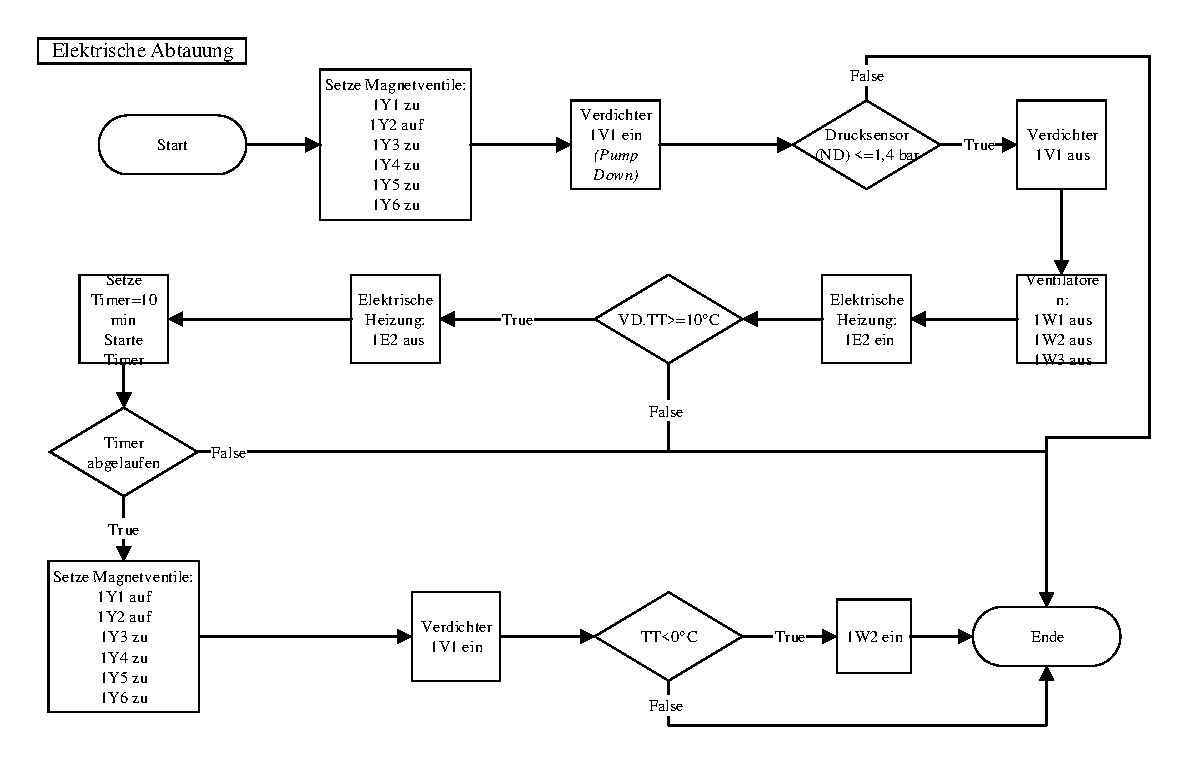
\includegraphics[ width=1.\textwidth]
{Pictures/Anhang/Ablauf_elektrisch.pdf}
\caption{Elektrische Abtauung}
\label{fig:}
\end{figure}

\chapter{Datenbank lesen}

\begin{figure}[htb]
\centering		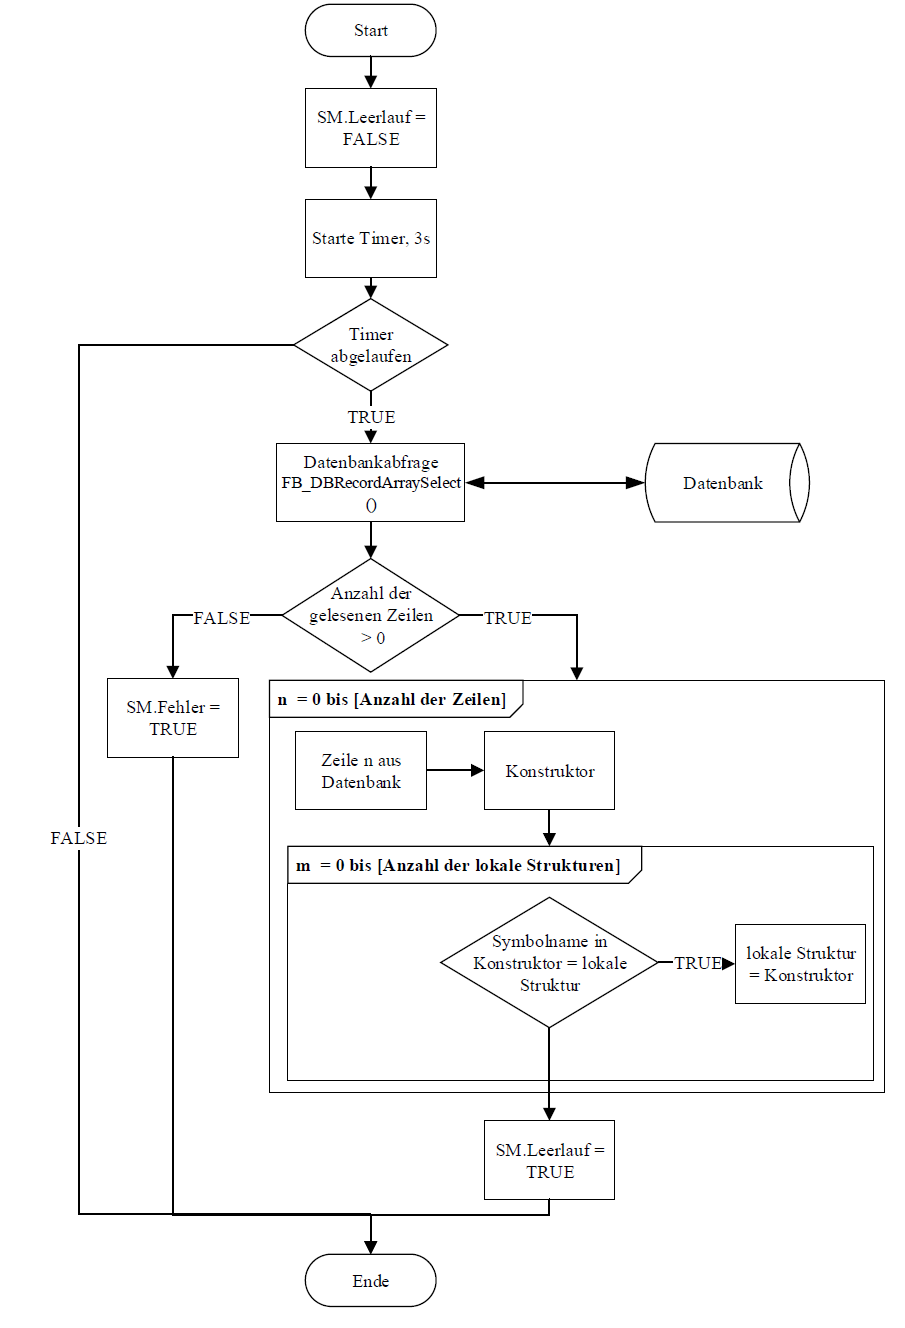
\includegraphics[width=0.650\textwidth]{Pictures/DB_lesen.png}
\caption{Initialisieren nach \citep{Nuerenberg2015}}
\label{fig:}
\end{figure}

\chapter{Software-Versionen}

\begin{table}[htb]
\centering
\caption{Benutzte Softwares und ihre Versionen}
\begin{tabular}{ll}
\hline 
\textbf{Programm} & \textbf{Version} \\ 
\hline 
\hline 
TwinCAT 3 & 3.1 Build 4020 \\ 
\hline 
TwinCAT 3 Database Konfigurator & 3.1.1.30 \\ 
\hline 
Microsoft Visual Studio Professional 2013 & 12.0.21005.1 REL \\ 
\hline 
MySQL Workbench & 6.3.6 \\ 
\hline 
\hline 
\end{tabular} 
\end{table}